%%%%%%%%%%%%%%%%%%%%%%%%%%%%%%%%%%%%%%%%%%%%%%%%%%%%%%
\section{A neural network determination of the ZLP}
%%%%%%%%%%%%%%%%%%%%%%%%%%%%%%%%%%%%%%%%%%%%%%%%%%%%%
\label{sec:methodology}

In this section we present our strategy to parametrise and subtract in a model-independent manner
the zero-loss peak that arises in the low-loss region of EEL spectra by means
of machine learning.
%
As mentioned in the introduction, our strategy will be inspired by the 
NNPDF method~\cite{Rojo:2018qdd} originally developed in the context of high-energy physics
for studies of the quark and gluon substructure of the proton~\cite{Gao:2017yyd}.
%
The NNPDF approach has been successfully applied, among others, to
the determination of
unpolarised~\cite{DelDebbio:2007ee,Ball:2008by,Ball:2012cx,Ball:2014uwa,Ball:2017nwa}
and polarised parton distributions functions of protons,  nuclear
parton distributions~\cite{AbdulKhalek:2019mzd,AbdulKhalek:2020yuc}, and the
fragmentation functions of partons into neutral and charged
hadrons~\cite{Bertone:2017tyb,Bertone:2018ecm}.

We note that recently several applications of machine learning
to transmission electron microscopy analyses 
in the context of material science have been
presented, see {\it e.g.}~\cite{Gordon:2020, Zhang:2019, Jany:2017, Ziatdinov:2017,10.1145/2834892.2834896,doi:10.1021/acsnano.7b07504,cite-key}.
%
Representative examples
include the automated identification
of atomic-level structural information~\cite{10.1145/2834892.2834896},
the extraction of chemical information
and defect classification~\cite{doi:10.1021/acsnano.7b07504},
and spatial resolution enhancement
using  using a generative adversarial network~\cite{cite-key}.
%
To the best of our knowledge, this is
the first time that neural networks are used as 
 unbiased
 background-removal interpolators
 and combined with Monte Carlo sampling to construct a faithful estimate
of the model uncertainties.

In this section
first of all we discuss the parametrisation of the ZLP in terms of neural networks.
%
We then review the Monte Carlo replica method used to estimate and propagate the
uncertainties to the input data to the model predictions.
%
Subsequently, we present our training strategy both in case of vacuum and of sample spectra,
and discuss how one can select the hyper-parameters that appear in the model.

\subsection{ZLP parametrisation}
\label{sec:parametrisation}

To begin with we note that, without any loss of generality, the intensity profile
associated to an EEL spectrum may be decomposed as
\be
\label{eq:IeelTot}
I_{\rm EEL}(\Delta E) =I_{\rm ZLP}(\Delta E) + I_{\rm inel}(\Delta E) \, ,
\ee
where $\Delta E$ is the measured electron energy loss; $I_{\rm ZLP}$ is the zero-loss peak
distribution arising both from instrumental origin  and from elastic scatterings; and
$I_{\rm inel}(\Delta E)$ contains the contributions from the
inelastic scatterings off the electrons and atoms in the specimen.
%
As shown by the representative example of Fig.~\ref{fig:EELS}, there are two limits
for which one can cleanly disentangle the two contributions.
%
First of all, for large enough values of
$\Delta E$ then
$I_{\rm ZLP}$ vanishes and thus $I_{\rm EEL} \to I_{\rm inel}$.
%
Secondly, in the $\Delta E\simeq 0$ limit all emission can be associated to
 the ZLP such that $I_{\rm EEL}\to  I_{\rm ZLP}$.
%
In this work we are interested in the ultra-low-loss region, where $I_{\rm ZLP}$ and $I_{\rm inel}$
become of the comparable magnitude.

Our goal is to construct a parametrisation of $I_{\rm ZLP}$ based on artificial
neural networks, which we denote by $I_{\rm ZLP}^{\rm (mod)}$, whereby we
can extract the relevant inelastic contribution by subtracting the
ZLP background to the measured intensity spectra,
\be
\label{eq:ZLPseparation}
I_{\rm inel}(\Delta E) \simeq I_{\rm EEL}(\Delta E) - I_{\rm ZLP}^{\rm (mod)}(\Delta E) \, ,
\ee
and thus be able to exploit the physical information contained in $I_{\rm inel}$ in
the low-loss region.
%
Crucially, we aim to faithfully estimate and propagate all the relevant sources of uncertainty associated
both to the input data and to methodological choices.

As discussed in Sect.~\ref{sec:eels}, the ZLP depends both
on the value of the electron energy loss $\Delta E$ as well as on the operation
parameters of the microscope, such as the electron beam energy $E_b$ and the exposure time
$t_{\rm exp}$.
%
Therefore we want to construct a multidimensional model which takes all relevant
variables as input.
%
This means that in general Eq.~(\ref{eq:ZLPseparation}) must be written as
\be
I_{\rm inel}(\Delta E) = I_{\rm EEL}(\Delta E, E_{b},t_{\rm exp}, \ldots) - I_{\rm ZLP}^{\rm (mod)}(\Delta E, E_{b},t_{\rm exp}, \ldots) \, ,
\ee
where we note that the subtracted spectra should depend only on $\Delta E$ but not on the microscope
operation parameters.
%
Ideally, the ZLP model should be able to accomodate as many input variables as possible.
%
Here we parametrise $I_{\rm ZLP}^{\rm (mod)}$ by means of
multi-layer feed-forward artificial neural networks, that is, we express our ZLP model as
\be
\label{eq:ZLPmodelNN}
I_{\rm ZLP}^{\rm (mod)}(\Delta E, E_{b},t_{\rm exp}, \ldots)  = \xi^{(n_l)}_1(\Delta E, E_{b},t_{\rm exp}, \ldots) \, ,
\ee
where $\xi^{(n_l)}_1$ denotes the activation state of the single neuron in the last
of the $n_l$ layers of the network when the $n_I$ inputs $\{ \Delta E, E_{b},t_{\rm exp}, \ldots \}$
are used.
%
The weights and thresholds of this neural network model are then determined
from the maximization of the model likelihood by means
of supervised learning and non-linear regression from a suitable training dataset.
%
This type of neural networks benefit from the ability
to parametrise multidimensional input data with arbitrarily
non-linear dependencies: even with a single hidden layer, a neural network
can reproduce arbitrary functional dependencies provided it has a large enough
number of neurons.

A schematic representation of our model
is displayed in Fig.~\ref{fig:architecture}.
%
 The input is an $n_I$ array containing $\Delta E$ and the rest of
 operation variables of the microscope, and
 the output is the value of the intensity of the ZLP distribution
 associated to those input variables.
 %
 We adopt an $n_I$-10-15-5-1 architecture with three hidden layers, for a total
 number of 289~(271) free parameters for $n_I=3$~($n_I=1$) to be adjusted by the optimization procedure.
 %
 We use a sigmoid activation function for the three hidden layers and a ReLU
 for the final one.
 %
 The choice of ReLU for the final layer guarantees that our model for the ZLP
 is positive-definite, as required by general physical considerations.
 %
 We have adopted a redundant architecture  to ensure that the ZLP parametrisation
 is sufficiently flexible, and we avoid over-fitting by means of
 a suitable regularisation strategy, see Sect.~\ref{sec:training}.
  
%%%%%%%%%%%%%%%%%%%%%%%%%%%%%%%%%%%%%%%%%%%%%
\begin{figure}[t]
    \centering
    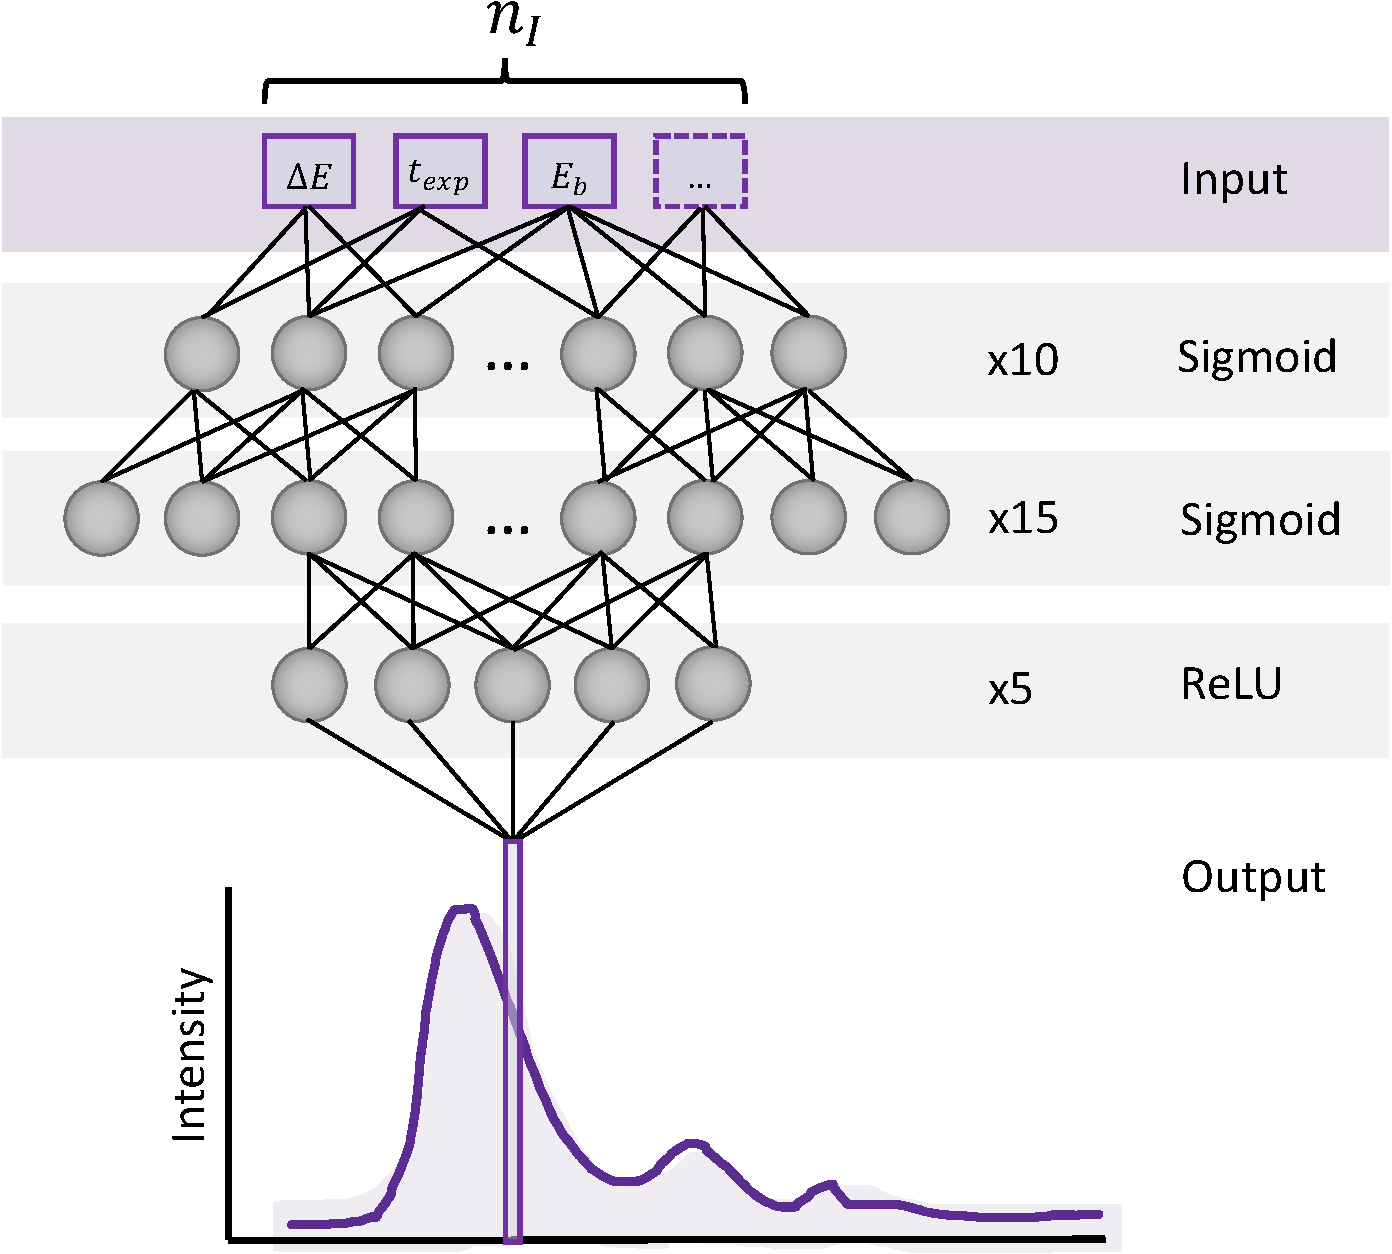
\includegraphics[width=99mm]{plots/architecture.pdf}
    \caption{Schematic representation of our ML model for the ZLP, Eq.~(\ref{eq:ZLPmodelNN}).
      %
      The input is an $n_I$-dimensional array containing $\Delta E$ and other
      operation variables of the microscope such as $E_b$ and $t_{\rm exp}$.
      %
      The output is the predicted value of the intensity of the zero-loss peak
      distribution associated to those specific input variables.
      %
      The architecture is chosen to be $n_I$-10-15-5-1, with sigmoid activation functions
      in all layers except for a ReLU in the output neuron.
    }
    \label{fig:architecture}
\end{figure}
%%%%%%%%%%%%%%%%%%%%%%%%%%%%%%%%%%%%%%%%%%%%%%%%%

\subsection{Uncertainty propagation}
\label{sec:MCreplicas}

We discussed in Sect.~\ref{sec:eels} how
even for EEL spectra taken at identical operation conditions of the microscope,
in general the resulting ZLP intensities will differ.
%
Further, there exist a large number of different NN configurations, each
representing a different functional form for $I_{\rm ZLP}^{(\rm mod)}$ which provide
an equally valid description of the input data.
%
To  estimate these uncertainties and propagate them to physical predictions,
we use here the Monte Carlo replica method.
%
The basic idea  is to exploit the available information
on experimental measurements (central values, uncertainties, and correlations)
to construct a sampling of the probability density in the space of 
the data, which by means of the NN training is then propagated
to a probability density in the space of $I_{\rm ZLP}$ models.

Let us assume that we have $n_{\rm dat}$ independent measurements of the ZLP intensity, for
different or the same values of the input parameters collectively denoted as $\{z_i\}$:
\be
I^{\rm (exp)}_{{\rm ZLP},i}\lp \{ z_i  \}\rp = I^{\rm (exp)}_{{\rm ZLP},i}\lp  \Delta E_i, E_{b,i}, t_{\rm exp,i},\ldots \rp
\,, \quad i=1,\ldots,n_{\rm dat} \, .
\ee
The Monte Carlo method is based on the generation
of a large number $N_{\rm rep}$ of Monte Carlo replicas of these original data points
by means of a multi-Gaussian distribution, with the central values and covariance matrices
from the input measurements,
\be
\label{eq:MCreplicaGen}
  I_{{\rm ZLP},i}^{{\rm (art)}(k)}  =  I^{\rm (exp)}_{{\rm ZLP},i} + r_i^{({\rm stat},k)}\sigma_i^{\rm (stat)}
  + \sum_{j=1}^{n_{\rm sys}} r_{i,j}^{({\rm sys},k)} \sigma_{i,j}^{\rm (\rm sys)} \,, \quad \forall i
  \,, \quad k=1,\ldots,N_{\rm rep} \,.\,\, \,
  \ee
  where $\sigma_i^{\rm (stat)}$ and $\sigma_{i,j}^{\rm (\rm sys)}$ represent the statistical
  and systematic uncertainties (the latter divided into  $n_{\rm sys}$ fully point-to-point correlated
  sources) and $\{r_i^{(k)}\}$ are Gaussianly distributed random numbers.
  %
  The values of $\{r_i^{(k)}\}$ are
  generated with a suitable correlation pattern to ensure
  that averages over the set of Monte Carlo
  replicas reproduce the original experimental covariance matrix, namely
  \be
  \la  \lp I_{{\rm ZLP},i}^{{\rm (art)}(k)} - \la I_{{\rm ZLP},i}^{{\rm (art)}}\ra_{\rm rep}\rp
  \lp I_{{\rm ZLP},j}^{{\rm (art)}(k)} - \la I_{{\rm ZLP},j}^{{\rm (art)}}\ra_{\rm rep}\rp\ra_{\rm rep}
  \label{eq:expcovariance} = {\rm cov}^{(\rm exp)}\lp I_{{\rm ZLP},i},I_{{\rm ZLP},j}\rp  \, ,
  \ee
  where averages are evaluated over the $N_{\rm rep}$ replicas that compose the sample.
  %
We thus note that each $k$-th replica contains 
as many data points as the original set.

In our case the information on experimental correlations is not accessible and
thus we assume that there is a single source of point-by-point uncorrelated systematic
uncertainty, denoted as $\sigma_i^{\rm (exp)}$, which is estimated as follows.
%
The input measurements will be composed in general on subsets of EEL
spectra taken with identical operation conditions.
%
Assume that for a specific set of operation conditions we have $N_{\rm sp}$ of such spectra.
%
Since the values of $\Delta E$ will be different in each case, first of all
we uniformise a common binning in $\Delta E$ with $n_{\rm dat}$ entries.
%
Then we evaluate the total experimental uncertainty in one of these bins as
\be
\label{eq:sigmaiexp}
\sigma_i^{\rm (exp)} = \lp \frac{1}{N_{\rm sp}-1} \sum_{l=1}^{N_{\rm sp}}
\lp I_{{\rm ZLP},i}^{ ({\rm exp}),l}  - \la I_{{\rm ZLP},i}^{ ({\rm exp})}\ra_{N_{\rm sp}} \rp \rp^{1/2} \, ,\,
i=1,\ldots, n_{\rm dat} \, ,
\ee
that is, as the standard deviation over the $N_{\rm sp}$ spectra.
%
This uncertainty is separately evaluated for each set of microscope operation conditions
for which data available.
%
In the absence of correlations Eqns.~(\ref{eq:MCreplicaGen}) and~(\ref{eq:expcovariance}) thus
simplify to
\be
 I_{{\rm ZLP},i}^{{\rm (art)}(k)}  =  I^{\rm (exp)}_{{\rm ZLP},i} + r_i^{({\rm tot},k)}\sigma_i^{\rm (exp)}
 \,, \quad \forall i
  \,, \quad k=1,\ldots,N_{\rm rep} \,.\,\, \,
\ee
and
  \bea
  \la  \lp I_{{\rm ZLP},i}^{{\rm (art)}(k)} - \la I_{{\rm ZLP},i}^{{\rm (art)}}\ra_{\rm rep}\rp
  \lp I_{{\rm ZLP},j}^{{\rm (art)}(k)} - \la I_{{\rm ZLP},j}^{{\rm (art)}}\ra_{\rep}\rp\ra_{\rm rep} =
  \sigma_i^{\rm (exp)}\sigma_j^{\rm (exp)}\delta_{ij} \, ,
  \eea
  given that the experimental covariance matrix is diagonal.
  %
  Should in the future correlations became available, it would be straightforward to extend
  our model to that case.

The value of the number of generated MC replicas, $N_{\rm rep}$, should be chosen such that the set of replicas 
models accurately the probability distribution of original training data.
%
To verify that this is the case,
Fig.~\ref{fig:MC} displays a comparison between the original experimental central values
$I_{{\rm ZLP},i}^{\rm (exp)}$ (left) and the corresponding 
total uncertainties $\sigma_i^{(\rm exp)}$ (right panel) with the results of averaging over
a sample of $N_{\rm rep}$ Monte Carlo replicas generated by means of
Eq.~(\ref{eq:MCreplicaGen}) for different number of replicas.
%
We find that $N_{\rm rep}=500$ is a value that ensures that both
the central values and uncertainties are reasonably well reproduced,
and we adopt it in what follows.

%%%%%%%%%%%%%%%%%%%%%%%%%%%%%%%%%%%%%%%%%%%%%%%
\begin{figure}[t]
    \centering
    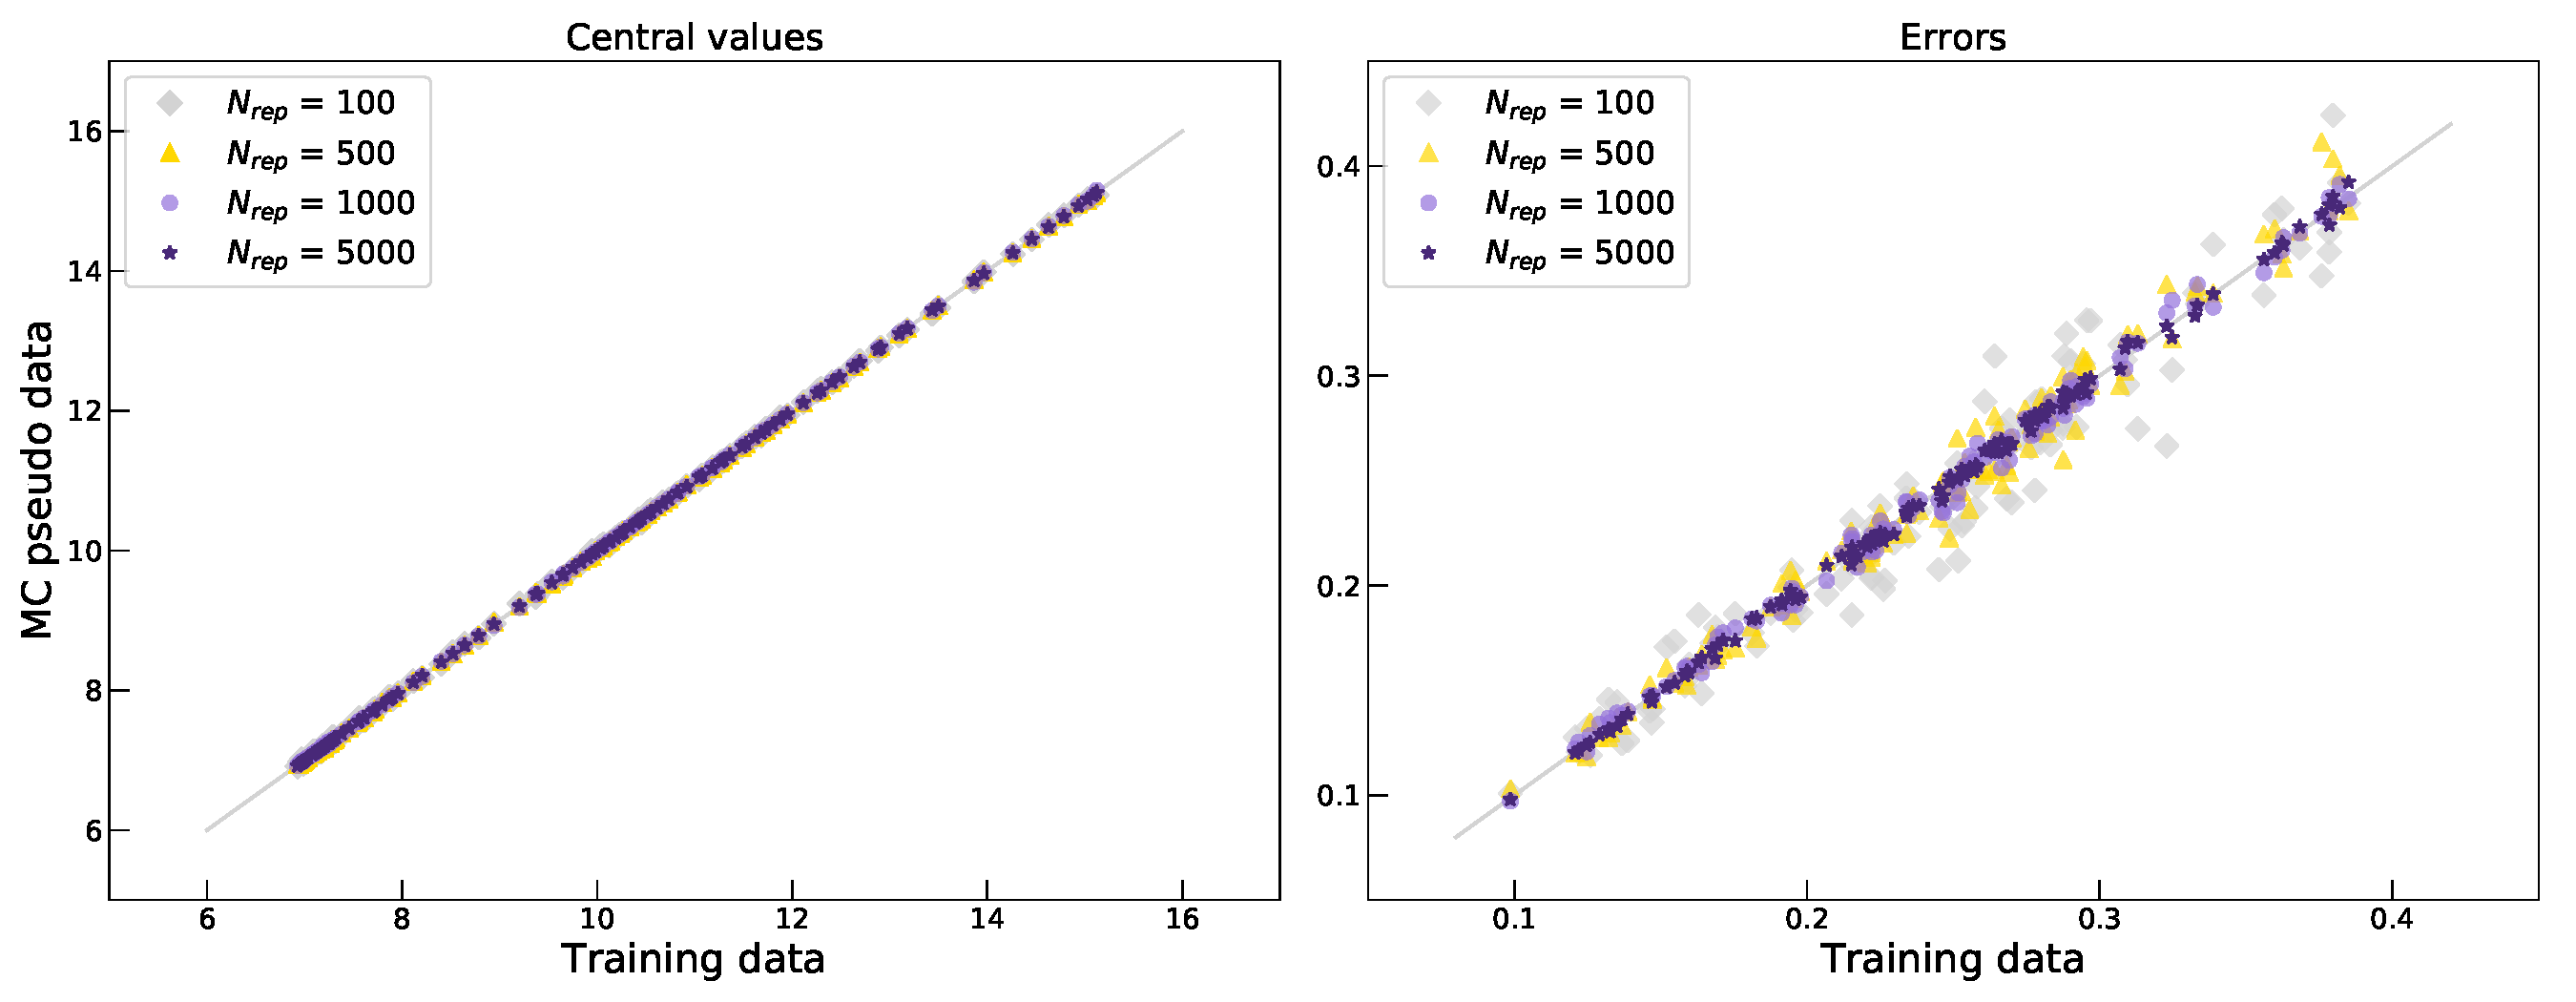
\includegraphics[width=0.99\textwidth]{plots/MC.pdf}
    \caption{Comparison between the original experimental central values
      $I_{\rm ZLP,i}^{\rm (exp)}$ (left) and the corresponding 
      uncertainties $\sigma_i^{(\rm exp)}$ (right panel) with the results of averaging over
      a sample of $N_{\rm rep}$ Monte Carlo replicas generated by means of
      Eq.~(\ref{eq:MCreplicaGen}), for different values of
      $N_{\rm rep}$.
      }
    \label{fig:MC}
\end{figure}
%%%%%%%%%%%%%%%%%%%%%%%%%%%%%%%%%%%%%%%%%%%%%%%%5

\subsection{Training strategy}
\label{sec:training}

The training of the neural network model for the ZLP peak differs between
the cases of EEL spectra taken on vacuum, where by construction $I_{\rm EEL}(\Delta E) =I_{\rm ZLP}^{\rm (mod)}(\Delta E)$,
and for spectra taken on specimens\footnote{Actually EEL spectra taken in the vacuum but close enough
  to the sample might still receive inelastic contributions from the specimen. In this work,
  when we use vacuum spectra, we consider exclusively those acquired reasonably far from the surfaces
of the analysed nanostructures.}.
%
In the latter case, as indicated by Eq.~(\ref{eq:ZLPseparation}), in order to avoid
biasing the results it is
important to ensure that the model is trained only on the region of the spectra
where the ZLP dominates over the inelastic scatterings.
%
We now describe the training strategy that is adopted in both cases.

\paragraph{Training of vacuum spectra.}
%
For each of the $N_{\rm rep}$ generated Monte Carlo replicas, we train an independent
neural network as described in Sect.~\ref{sec:parametrisation}.
%
The parameters of the neural network are determined from the minimisation of a figure of merit (the cost function of the model)
defined as
\begin{equation}
  \label{eq:chi2}
\begin{centering}
  E^{(k)}\lp \{\theta^{(k)}\}\rp = \frac{1}{n_{\rm dat}}\sum_{i=1}^{n_{\rm dat}}\left(\frac{ I_{{\rm ZLP},i}^{{\rm (art)}(k)} -
  I_{{\rm ZLP},i}^{{\rm (mod)}}\lp \{\theta^{(k)}\}\rp }{\sigma_i^{(\rm exp)}}\right)^2, 
\end{centering}
\end{equation}
which is the $\chi^2$ per data point comparing the $k$-th replica for the ZLP
intensity with the corresponding model prediction for the values
$\{\theta^{(k)}\}$ of its weights and thresholds.
%
In order to speed up the neural network training process, prior to the optimisation
all inputs and outputs are scaled to lie between $[0.1, 0.9]$ before
being feed to the network.
%
This preprocessing facilitates that
 the neuron activation states will typically
lie close to the linear region of the sigmoid activation function.

The contribution to the figure of merit from the input experimental data, Eq.~(\ref{eq:chi2}),
needs in general to be complemented with that of theoretical constraints on the model.
%
For instance, when determining nuclear parton distributions~\cite{AbdulKhalek:2020yuc}, one needs to
extend Eq.~(\ref{eq:chi2}) with Lagrange multipliers to ensure that both the $A=1$ proton boundary
condition and the cross-section positivity are satisfied.
%
In the case at hand, our model for the ZLP should implement the property that $I_{\rm ZLP}(\Delta E)\to 0$
when $|\Delta E| \to \infty$, since far from $\Delta E\simeq 0$ the contribution from elastic scatterings
and instrumental broadening is completely negligible.
%
In order to implement this constraint, we add $n_{\rm pd}$ pseudo-data points to the training dataset and modify
the figure of merit Eq.~(\ref{eq:chi2}) as follows
\be
\label{eq:chi2modified}
E^{(k)}\lp \{\theta^{(k)}\}\rp \to E^{(k)}\lp \{\theta^{(k)}\}\rp +
\lambda \sum_{i'=1}^{n_{\rm pd}}\left(
  I_{{\rm ZLP},i'}^{{\rm (mod)}}\lp \{\theta^{(k)}\}\rp \right)^2, 
  \ee
  where $\lambda$ is a Lagrange multiplier whose value is tuned to ensure that the $I_{\rm ZLP}(\Delta E)\to 0$
  condition
  is satisfied without affecting the description of the training dataset.
  %
  The pseudo-data points are chosen to lie in the region $[\Delta E_{\rm pd}^{\rm (min)},
  \Delta E_{\rm pd}^{\rm (max)}]$ (and symmetrically for negative energy losses).

  %
  The value of $\Delta E_{\rm pd}^{\rm (min)}$
  is determined automatically by evaluating the ratio of the intensity to the uncertainty in each data point, 
  $I_{{\rm ZLP},i}^{(\rm exp)} / \sigma_{i}^{(\rm exp)}$. 
  %
  At a certain energy loss this ratio approaches unity, which indicates that one is essentially fitting statistical noise.
  %
  In order to avoid this and only fit data that is different from zero within errors, we
  determine $\Delta E_{\rm pd}^{\rm (min)}$ as the value of $\Delta E$
  for which the ratio  $I_{{\rm ZLP},i}^{(\rm exp)} / \sigma_{i}^{(\rm exp)}$  becomes unity.
  %
  We then maintain the training data in the region $\Delta E \le \Delta E_{\rm pd}^{\rm (min)}$ and the pseudo-data
  points are added for $[ \Delta E_{\rm pd}^{\rm (min)}, \Delta E_{\rm pd}^{\rm (max)}]$. 
  %
  The value of $\Delta E_{\rm pd}^{\rm (max)}$ can be chosen arbitrarily and can be as large as necessary
  to ensure that $I_{\rm ZLP}(\Delta E)\to 0$ as $|\Delta E| \to \infty$.
  %u
We note that another important physical condition on the ZLP model, namely its positivity
(since in EEL spectra the intensity is just a measure of the number of counts in the
detector for a given value of the energy loss) is automatically satisfied since
we use a ReLU activation function for the last layer.

In this work we adopt the {\tt TensorFlow} library to assemble
the architecture illustrated in  Fig.~\ref{fig:architecture}.
%
Before training, all weights and biases are initialized in a non-deterministic order
by the built-in global variable initializer. 
%
The optimisation of the figure of merit Eq.~(\ref{eq:chi2modified}) is carried
out by means of stochastic gradient descent (SGD) combined with backpropagation, specifically
by means of the Adam minimiser.
%
The hyper-parameters of the optimisation algorithm such as the learning rate
have been adjusted to ensure proper learning is reached in the shortest amount
of time possible.

Given that we have a extremely flexible parametrisation, one should be careful
to avoid overlearning the input data.
%
Here over-fitting is avoided by means of a cross-validation stopping criterion.
%
We separate the input data into training a validation subsets, with a 80\%/20\% splitting
which varies randomly for each Monte Carlo replica.
%
We then run the optimiser for a very large number of iterations and store both
the state of the network and the value
of the figure of merit Eq.~(\ref{eq:chi2}) restricted to the validation
dataset, $E^{(k)}_{\rm val}$ (which is not used for the training).
%
The optimal stopping point is then determined {\it a posteriori} for each replica
as the specific network configuration that leads to the deepest minimum of $E^{(k)}_{\rm val}$.
%
The number of epochs should be chosen high enough to reach the optimal stopping point for each replica.
%
In this work we find that $40k$ epochs are sufficient to be able to identify these optimal stopping points.
%
This corresponds to a serial running time of 
$t\simeq 60$ seconds per replica when running the optimization on a  single CPU for 500 datapoints.

Once the training of the $N_{\rm rep}$ neural network models for the ZLP has been carried
out as specified above, we gauge the overal fit quality of the model by computing the
$\chi^2$ defined as
\begin{equation}
  \label{eq:chi2_final}
\begin{centering}
  \chi^2 = \frac{1}{n_{\rm dat}}\sum_{i=1}^{n_{\rm dat}}\left(\frac{ I_{{\rm ZLP},i}^{{\rm (exp)}} -
 \la I_{{\rm ZLP},i}^{{\rm (mod)}}\ra_{\rm rep} }{\sigma_i^{(\rm exp)}}\right)^2, 
\end{centering}
\end{equation}
which is the analog of Eq.~(\ref{eq:chi2_final}) now comparing the average model prediction
to the original experimental data values.
%
A value $\chi^2 \simeq 1$ indicates that a satisfactory description of the experimental data,
within the corresponding uncertainties, has been achieved.
%
Note that in realistic scenarios $\chi^2$ can deviate from unity, for instance when
some source of correlation between the experimental uncertainties has been neglected, or on the contrary
when the total experimental error is underestimated.

\paragraph{Training of sample spectra.}

The training strategy in the case of EEL spectra acquired on specimens (rather than on vacuum) must be adjusted
to account for the fact that the input data set, Eq.~(\ref{eq:IeelTot}), receives contributions
both from the ZLP and from inelastic scatterings.
%
To avoid biasing the ZLP model, only the former contributions should be
included in the training dataset.

We can illustrate the situation here with the help of a simple toy model for the low-loss
region of EEL spectra, represented in
Fig.~\ref{fig:EELS_toy}.
%
Let us assume that the ZLP is described by a Gaussian distribution with a standard deviation of $\sigma_{\rm ZLP}=0.3$ eV,
and that the contribution from the
inelastic scatterings arising from the sample can be approximated in the low-loss
region by $I_{\rm inel}(\Delta E)\propto \lp \Delta E - E_{\rm bg}\rp^b$ with $E_{\rm bg}=1.5$ eV
and $b=1/2$.
%
The motivation for this
choice will be spelled out in Sect.~\ref{sec:results_sample}.
%
We display the separate contributions from $I_{\rm ZLP}$
and $I_{\rm inel}$, as well as their sum, 
with the inset showing the values of the corresponding derivatives, $dI/d\Delta E$.

%%%%%%%%%%%%%%%%%%%%%%%%%%%%%%%%%%%%%%%%%%%%%
\begin{figure}[t]
    \centering
    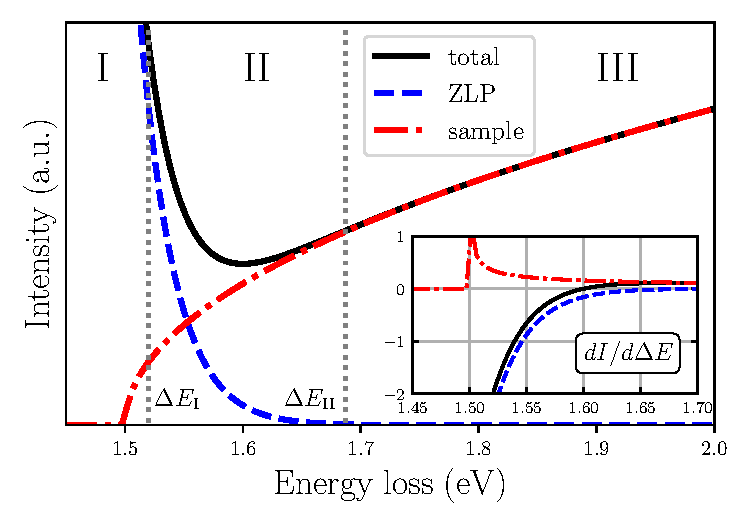
\includegraphics[width=0.89\textwidth]{plots/EELS_toy.pdf}
    \caption{A toy model for the EEL spectrum and its
      derivative (in the inset).
      %
      We display the separate contributions from $I_{\rm ZLP}$
      and $I_{\rm inel}$ as well as their sum.
      %
      We indicate the two regions used for the model training ($\rm I$ and $\rm III$),
      while as discussed in the text the trained model is then
      extrapolated to region $\rm II$, defined for $\Delta E_{\rm I} \le \Delta E \le \Delta E_{\rm II}$.
    }
    \label{fig:EELS_toy}
\end{figure}
%%%%%%%%%%%%%%%%%%%%%%%%%%%%%%%%%%%%%%%%%%%%%%%%%

The simple toy model of Fig.~\ref{fig:EELS_toy} is general enough so that one can draw
a number of useful considerations concerning the relation between $I_{\rm ZLP}$ and $I_{\rm inel}$
that will apply also in realistic spectra:

\begin{itemize}

\item The ZLP intensity, $I_{\rm ZLP}(\Delta E)$, is a monotonically decreasing function
  and thus its derivative is always negative.

\item  The first local minimum of the total intensity, $dI_{\rm EEL}/d\Delta E|_{\Delta E_{\rm min}}=0$, corresponds
  to a value of $\Delta E$ for which the contribution from the inelastic emissions is already
  sizable.

\item The value of $\Delta E$ for which $I_{\rm inel}$ starts to contribute to the total spectrum
  corresponds to the position where the intensity derivatives in-sample and in-vacuum  start to differ.
  %
  We note that a direct comparison between the overal magnitude of the sample and vacuum ZLP
  spectra is in general not possible, as explained in Sect.~\ref{sec:eels}. 
\end{itemize}

These considerations suggest that when training the ML model on EEL spectra taken on samples,
the following categorisation should de adopted:

\begin{enumerate}

\item For energy losses such that $\Delta E \le \Delta E_{\rm I}$ (region $\rm I$),
  the model training  proceeds in the same way as for the vacuum case
  via the minimisation of Eq.~(\ref{eq:chi2})

\item  
  For $\Delta E \ge \Delta E_{\rm II}$ (region $\rm III$), we use instead Eq.~(\ref{eq:chi2modified})
  without the contribution from the input data, since for such values
  of $\Delta E$ one has that $I_{\rm inel}\gg I_{\rm ZLP}$.
  %
  In other words, the only information that the region $\rm III$ provides
  on the model is the one arising from the implementation
  of the constraint that $I_{\rm ZLP}(\Delta E\to \infty)\to 0$.

\item The EELS data  in region $\rm II$, defined by  $\Delta E_{\rm I} \le \Delta E \le \Delta E_{\rm II}$,
  is excluded from the training dataset, given that in this region the contribution to $I_{\rm EEL}$
  coming from $I_{\rm inel}$ is significant.
  %
  There the model predictions are obtained from an interpolation
  of the associated predictions obtained in the regions $\rm I$ and $\rm III$.

\end{enumerate}

This classification introduces two new hyper-parameters of our model, $\Delta E_{\rm I}$ and
$\Delta E_{\rm II}$, which need to be specified before the training.
%
They should satisfy $\Delta E_{\rm I} \le \Delta E_{\rm min}$ and $\Delta E_{\rm II} \ge \Delta E_{\rm min}$,
with $\Delta E_{\rm min}$ being the position of the first local minimum of $I_{\rm EEL}$.
%
As indicated by the toy spectra of Fig.~\ref{fig:EELS_toy}, a suitable value for $\Delta E_{\rm I}$
would be somewhat above the onset of the inelastic contributions, to maximise
the amount of training data while ensuring that $I_{\rm EEL}$ is dominated
by $I_{\rm ZLP}$.

The optimal value of $\Delta E_{\rm I}$  can be determined as follows.
%
We evaluate the ratio
between the derivative of the intensity distribution acquired on the specimen over the
same quantity recorded in vacuum,
\be
\label{eq:rder}
\mathcal{R}^{(j)}_{\rm der}(\Delta E) \equiv
\la
\frac{
  dI_{\rm EEL}^{({\rm exp})(j)}(\Delta E)/ d\Delta E
}{
  dI_{\rm EEL}^{({\rm exp})(j')}(\Delta E) /d\Delta E
} \ra_{N_{\rm sp}' } \, ,
\ee
where $j'$ labels one of the $N_{\rm sp}'$ vacuum spectra and the average is taken
over all available values of $j'$.
%
This ratio allows one to identify a suitable value of $\Delta E_{\rm I}$ by establishing
for which energy losses the shape (rather than the absolute value) of the intensity distributions 
recorded on the specimen starts to differ significantly from their vacuum counterparts.
%
A sensible choice of $\Delta E_{\rm I}$ could for instance be given by
$\mathcal{R}_{\rm der}(\Delta E_{\rm I}) \simeq 0.8$, for which derivatives differ
at the 20\% level.
%
Note also that the leftmost value of the energy loss satisfying
$\mathcal{R}_{\rm der}(\Delta E)=0$ in Eq.~(\ref{eq:rder}) corresponds to the position of the first
local minimum.
